\chapter{Základné pojmy}



%%%%%%%%%%%%%%%%%%%%%%%%%%%%%%%%%%%%%%%%%%%%%%%%%%%%%%%%%%%%%%%%%%%%%%%%%%%%%%%%%%%%%%%%%%%%%%%%%%%%%%%%%%%%%%%%%%%%%%%%%%%%%%%%%%%%%%%%%%%%%%%%%%%%%%%%%%%%%%%%%%%%%%%%%%%%%%%%%%%%%%%%%%%%%%%%%%%%%%%%%%%%%%%%%%%%%%%%%%%%%%%%%%%%%%%%%%%%%%%%%%%%%%%%%

\section{\acs{HTML} 5 štandardy}

Medzi štandardy ... 

Na obrázku \ref{fig:obrazokHTML} sú HTML5 rozhrania API a súvisiace technológie taxonómie a status

\begin{figure}
\centering
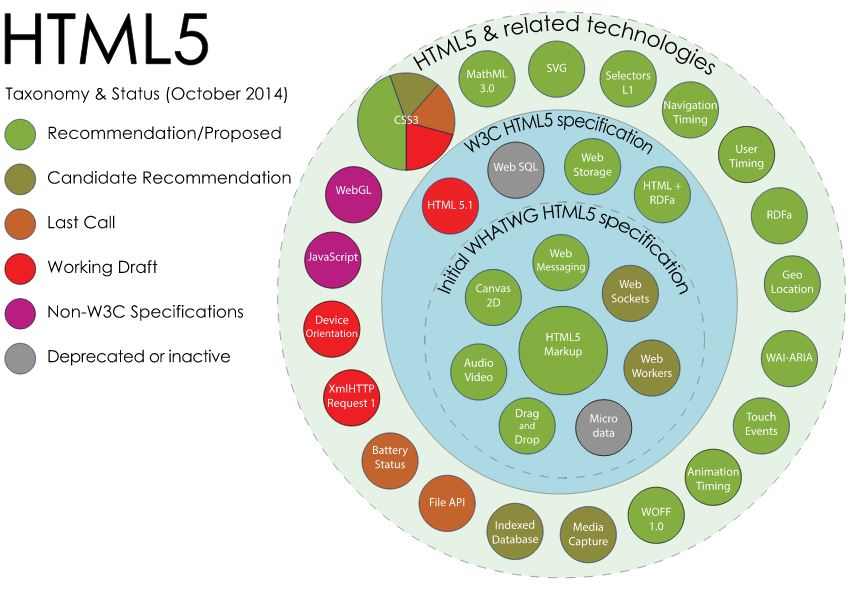
\includegraphics[width=0.7\linewidth]{obrazky/obrazokHTML}
\caption{HTML 5 API}
\label{fig:obrazokHTML}
\end{figure}
%http://html5.belisso.com/




%\ac*{W3C} značkový jazyk vždy bolo \acs{HTML}. 
%HTML bolo primárne navrhnuté ako jazyk, pre systematické opisovanie vedeckých dokumentov.  
%Hlavná oblasť
%TODO

%http://www.w3.org/TR/html5/  

%The World Wide Web's markup language has always been HTML. HTML was primarily designed as a language for semantically describing scientific documents, although its general design and adaptations over the years have enabled it to be used to describe a number of other types of documents.

%The main area that has not been adequately addressed by HTML is a vague subject referred to as Web Applications. This specification attempts to rectify this, while at the same time updating the HTML specifications to address issues raised in the past few years.

%1.2 Audience

%This section is non-normative.

%This specification is intended for authors of documents and scripts that use the features defined in this specification, implementors of tools that operate on pages that use the features defined in this specification, and individuals wishing to establish the correctness of documents or implementations with respect to the requirements of this specification.

%This document is probably not suited to readers who do not already have at least a passing familiarity with Web technologies, as in places it sacrifices clarity for precision, and brevity for completeness. More approachable tutorials and authoring guides can provide a gentler introduction to the topic.

%In particular, familiarity with the basics of DOM is necessary for a complete understanding of some of the more technical parts of this specification. An understanding of Web IDL, HTTP, XML, Unicode, character encodings, JavaScript, and CSS will also be helpful in places but is not essential.

%1.3 Scope
%
%This section is non-normative.

%This specification is limited to providing a semantic-level markup language and associated semantic-level scripting APIs for authoring accessible pages on the Web ranging from static documents to dynamic applications.

%The scope of this specification does not include providing mechanisms for media-specific customization of presentation (although default rendering rules for Web browsers are included at the end of this specification, and several mechanisms for hooking into CSS are provided as part of the language).

%The scope of this specification is not to describe an entire operating system. In particular, hardware configuration software, image manipulation tools, and applications that users would be expected to use with high-end workstations on a daily basis are out of scope. In terms of applications, this specification is targeted specifically at applications that would be expected to be used by users on an occasional basis, or regularly but from disparate locations, with low CPU requirements. Examples of such applications include online purchasing systems, searching systems, games (especially multiplayer online games), public telephone books or address books, communications software (e-mail clients, instant messaging clients, discussion software), document editing software, etc.

%1.4 History


%
%blal 3.2.5.1 The id attribute
%
%The id attribute specifies its element's unique identifier (ID). [DOM]
%
%The value must be unique amongst all the IDs in the element's home subtree and must contain at least one character. The value must not contain any space characters.





\section{Čo je SVG?}
\ac{SVG} je štandardný formát pre vektorovú grafiku. Vektorová grafika je definovaná cez body, priamky, mnohouholníky, elipsy, krivky, alebo iné geometrické tvary.  

\acs{SVG} je jazyk na opísanie dvojrozmernej grafiky v   \ac*{XML}. Vďaka tomu, umožňuje reprezentáciu grafických informácii v kompaktnom a prenositeľnom tvare.
%SVG patrí do rodiny špecifikácií HTML 5.

 SVG povoľuje tieto tri typy grafických objektov: vektorové grafické tvary, obrázky a text. 
Grafické objekty môžu byť zoskupené, štylizované, zmenené, a kombinované do predošlých vrstiev objektov. 

SVG obrázky môžu byť dynamické a interaktívne. \ac*{DOM} pre SVG, ktoré zahŕňa celé XML DOM, a povoľuje priamočiaro a efektívnu vektorovú grafickú animáciu cez príkazy. TODO

Prispôsobiteľnosť SVG umožňuje zmeniť veľkosť grafického komponentu bez straty kvality vzhľadu. Čo umožňuje zobraziť responzívne na viacerých možných zariadení. 
SVG sa bude zobrazovať rovnako na rôznych platformách. Je kompatibilná s štandardmi \acs{HTML}5, ktoré navrhla \ac*{W3C}. 

%http://www.w3.org/Graphics/SVG/About.html

%SVG is a language for describing two-dimensional graphics in XML. SVG allows for three types of graphic objects: vector graphic shapes (e.g., paths consisting of straight lines and curves), images and text. Graphical objects can be grouped, styled, transformed and composited into previously rendered objects. Text can be in any XML namespace suitable to the application, which enhances searchability and accessibility of the SVG graphics. The feature set includes nested transformations, clipping paths, alpha masks, filter effects, template objects and extensibility.

%SVG drawings can be dynamic and interactive. The Document Object Model (DOM) for SVG, which includes the full XML DOM, allows for straightforward and efficient vector graphics animation via scripting. A rich set of event handlers such as onmouseover and onclick can be assigned to any SVG graphical object. Because of its compatibility and leveraging of other Web standards, features like scripting can be done on SVG elements and other XML elements from different namespaces simultaneously within the same Web page.
 
 
 \subsection{Podpora v webovom prehliadači}
 Súčasné prehliadače plne podporujú SVG elementy.
 V tabuľke je TODO - PREROBIM TO ESTE DO TABULKY 
 \begin{figure}
\centering
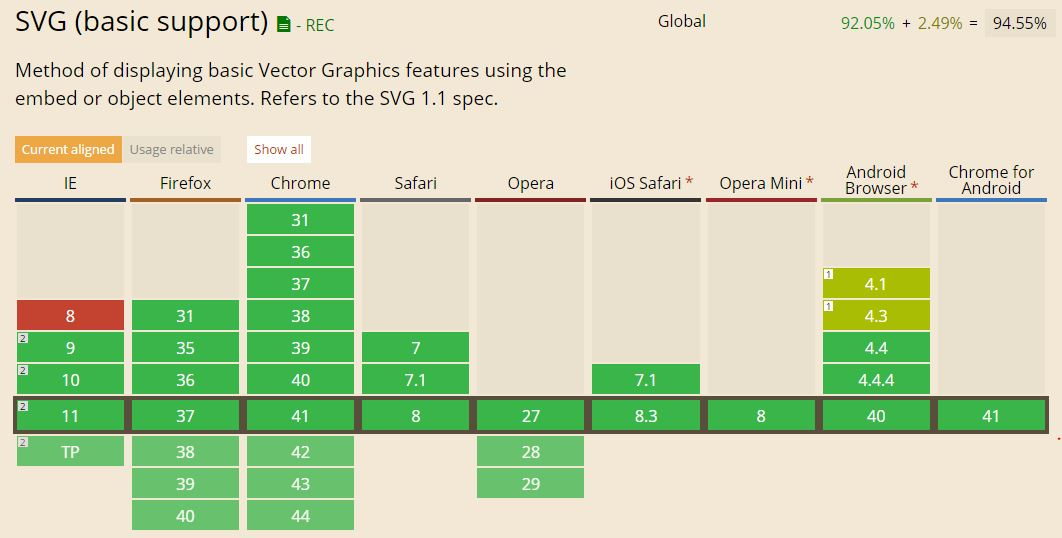
\includegraphics[width=0.7\linewidth]{obrazky/podpora}
\caption{podpora SVG vo webových prehliadačoch}
\label{fig:podpora}
\end{figure}

 
% http://caniuse.com/#feat=svg
 
 \subsection{Rozdiely medzi SVG a Canvas}
TODO \url{http://www.petrpexa.cz/diplomky/trantyr.pdf} strana 52


 SVG je jazyk na opisanie dvojrozmernej grafiky v XML. 
 Canvas kreslí dvojrozmernú grafiku za behu programu cez JavaScript.
 SVG je XML založený, čo znamená, že každý element je dostupný cez SVG DOM. Môžem k tomu priložiť JavaScript na ovládanie udalostí elementov. TODO . 
  %You can attach JavaScript event handlers for an element.
 V SVG je každý tvar zapamätaný ako objekt. Ak potrebujem zmeniť atribút SVG, tak prehliadač  automaticky prekreslí daný tvar.
 
 
 Canvas je prekresľovaný pixel za pixelom. Prehliadač na neho zabudne, ako náhle sa vykreslí. Keď chcem zmeniť jeho pozíciu, musím prekresliť úplne všetko. 
 
 
 %SVG is XML based, which means that every element is available within the SVG DOM. You can attach JavaScript event handlers for an element.
 %In SVG, each drawn shape is remembered as an object. If attributes of an SVG object are changed, the browser can automatically re-render the shape.
 %Canvas is rendered pixel by pixel. In canvas, once the graphic is drawn, it is forgotten by the browser. If its position should be changed, the entire scene needs to be redrawn, including any objects that might have been covered by the graphic.
 
 
 \subsection{Porovnanie Canvas a SVG}
 Tabuľka \ref{canvas:SVG} zobrazuje niekoľko dôležitých odlišností medzi Canvas a SVG. 
% The table below shows some important differences between Canvas and SVG:
 TODO DPI
 \begin{table}[h]
 \centering
 \begin{tabular}{|l|p{7.5cm} |}
 	\hline \textbf{Canvas} & \textbf{SVG} \\
 	 	\hline Závislé na rozlíšení a \acs{DPI} & Nezávislé na rozlíšení a DPI \\ 
 	\hline Nepodporuje dynamické zmeny & Podporuje dynamické zmeny \\ 
 	\hline Obmedzené možnosti na vykresľovanie  & Vhodné pre aplikácie s veľkými plochami na vykresľovanie \\ 
 	\hline & Väčší výpočtový výkon pri komplexnom obrázku \\ 
 	\hline Vhodné pre grafické-intenzívne hry & Nevhodné pre dynamické hry \\ 
 	\hline 
 \end{tabular} 

 \caption{Porovnanie Canvas a SVG}
 \label{canvas:SVG}
 
\end{table}
 
 
 \section{Základná syntax \acs*{SVG}}
TODO
V HTML5 sa môžu používať vložené SVG elementy priamo v na HTML stránke. 
%https://css-tricks.com/using-svg/

%TODO DOPLNIT POUTIZIIE TRI SPOSOBY \url{https://css-tricks.com/using-svg/}

SVG can be created 
-   inline: within the HTML document 
-   by embedding a stand alone .SVG file


Copy/paste SVG code within HTML code (inlining)
Using the HTML img tag
Using the HTML object tag
Using the HTML iframe tag
Using CSS (background images)
Including SVG within SVG using the image tag.


%citovane z knihy Sergey's HTML5 & CSS3 Quick Reference: HTML5, CSS3 and APIs (3rd Edition)
%preview je volne dostupny na nete / aspon tie kapitoly, ktore potrebujem


\begin{table}[h]
	\begin{center}
		\begin{tabular}{|l|l|}
			\hline \textbf{Technika} & \textbf{Popis} \\ 
			\hline $<$embed$>$ tag & Načíta vytvorený SVG súbor.  \\ 
			\hline $<$object$>$ tag & Nepovoľuje skriptovanie.  \\ 
			\hline $<$iframe$>$ tag & Zobrazí SVG v rámci  \\ 
			\hline Inline & Vytvorí Svg súbor \\ 
			\hline 
		\end{tabular} 
	\end{center}
	\caption{Spôsoby vytvorenia SVG v HTML dokumente}
	\label{vytvorenie:SVG}
\end{table}

Príklady načítania SVG v HTML dokumente.

$<$img$>$ tag 

\begin{lstlisting}
	Image:
	<img src="stanica2.svg" width = "50" height= "50" />
	
	Embed:
	<embed src="stanica2.svg" width = "50" height= "50" />
	
	Object:
	<object type="image/svg+xml" data="stanica2.svg"
	width="50" height="50"></object>
	
	Iframe:
	<iframe src="stanica2.svg" width = "50" height= "50"><</iframe>
	
\end{lstlisting}






\subsection{Príklad použitia SVG v HTML dokumentu s inline SVG }

HTML kód: 

\begin{lstlisting}
<!DOCTYPE html>
<html>
<head lang="sk">
<meta charset="UTF-8">
<title></title>
</head>
<body>

	<svg width="100" height="100">
		<circle cx="50" cy="50" r="40" stroke="black" stroke-width="2" fill="silver" />
	</svg>	
	
</body>
</html>

\end{lstlisting}




SVG obrázok začína s $<$svg$>$ elementom. Atribúty elementu $<$svg$>$ sú width a height. Definujú šírku a výšku SVG obrázka. Element $<$circle$>$ je použitý na nakreslenie kruhu. Atribúty cx, cy definujú x, y súradnice od centra kruhu. Ak je cx, cy vynechané, tak center kruhu je nastavený na $($0, 0$)$. Atribút r  definuje polomer kruhu. Atribúty stroke a stroke-width určujú to ako bude vyzerať obrys útvaru. Kruh má nastavený 2px čierny okraj. 
Atribút fill vyplní vnútro kruhu. V príklade je vyplnený sivou farbou. Tag, ktorý uzavrie SVG obrázok je $<$$/$svg$>$. Keďže SVG je validné XML, tak všetky elementy musia byť správne zatvorené. 
%zdroj www.w3schools.com/svg/svg_inhtml.asp


Vykreslí na HTML webovú stránku útvar, ktorý je na obrázku \ref{jednoduchyKruh}.

\begin{figure}[ht]
	\begin{center}
		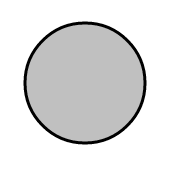
\includegraphics  {obrazky/jednoduchyKruh.png}
		\caption{Vykreslenie SVG na HTML stránke}
		\label{jednoduchyKruh}
	\end{center}
\end{figure}


\section{SVG útvary} 

\acs*{SVG} má preddefinované tieto tvary elementov:
\begin{itemize}
	\item Obdĺžník $<$rect$>$
	\item Kruh $<$circle$>$
	\item Elipsa $<$ellipse$>$
	\item Čiara $<$line$>$
	\item Polyline $<$polyline$>$
	\item Mnohouholník $<$polygon$>$
	\item Cesta $<$path$>$	
\end{itemize}

TODO ESTE NIECO PRIDAT

%\section{CSS vlastnosti - tuto kapitolu asi vyhodim}
%
%Podľa HTML5 štandardov dokáže CSS meniť vlastnosti SVG.
%
%%www.w3.org/tr/svg/styling.html
%%http://www.w3.org/TR/SVG/propidx.html http://www.w3.org/TR/SVG2/styling.html
%
%Vymenované vlastnosti, ktoré majú rovnaké \acs{CSS} 2.1 a \acs{SVG}. 
%
%Vlastnosti písma: 
%‘font’,
%‘font-family’,
%‘font-size’,
%‘font-size-adjust’,
%‘font-stretch’,
%‘font-style’,
%‘font-variant’,
%‘font-weight’.
%
%Vlastnosti textu: 
%‘direction’,
%‘letter-spacing’,
%‘text-decoration’,
%‘unicode-bidi’,
%‘word-spacing’.
%
%Ďalšie vlastností:
%‘clip’,
%‘color’ (‘fill’, ‘stroke’, ‘stop-color’, ‘flood-color’ a ‘lighting-color’), 
%‘cursor’,
%‘display’,
%‘overflow’,
%‘visibility’.
%
%Nasledujúce vlastností nie sú definované v CSS 2.1. 
%
%Clipping, Masking and Compositing properties:
%‘clip-path’, 
%‘clip-rule’,
%‘mask’, 
%‘opacity’.
%
%
%Filter Effects properties:
%‘enable-background’
%‘filter’
% ‘flood-color’
% ‘flood-opacity’
% ‘lighting-color’	
%
%
%Gradient properties: ‘stop-color’, 	‘stop-opacity’. 
%
%Interactivity properties:
%\begin{itemize}
%\item 	‘pointer-events’
%\end{itemize}
%Color and Painting properties:
%\begin{itemize}
%\item ‘color-interpolation’, ‘color-rendering’
%\item ‘fill’, ‘fill-opacity’, ‘fill-rule’
%\item ‘image-rendering’
%\item ‘marker’, ‘marker-end’, ‘marker-mid’,‘marker-start’
%\item ‘shape-rendering’
%\item ‘stroke’, ‘stroke-dasharray’, ‘stroke-dashoffset’, ‘stroke-linecap’, ‘stroke-linejoin’, ‘stroke-miterlimit’, ‘stroke-opacity’, ‘stroke-width’
%\item ‘text-rendering’	
%\end{itemize}
%
%Text properties:
%\begin{itemize}
%\item 	‘alignment-baseline’
%\item 	‘baseline-shift’
%\item 	‘dominant-baseline’
%\item 	‘glyph-orientation-horizontal’
%\item 	‘glyph-orientation-vertical’
%\item 	‘text-anchor’
%\item 	‘writing-mode’
%\end{itemize}
%
% 
%
%mozno tu este pridam nieco z prezentacii, ktore ma ucitel mikus
